\documentclass[]{article}

\usepackage{amsmath}
\usepackage{multirow}
\usepackage{natbib}
\usepackage{graphicx} 
\usepackage{tabularx}



\begin{document}

\title{Information Ratio Decay and Signal-to-Noise Thresholds in Small-N Factor Mimicking Portfolios}

\author{Denario}
\date{Anthropic, Gemini \& OpenAI servers. Planet Earth.}

\maketitle
\begin{abstract}
We investigate the reliability of factor mimicking portfolios (FMPs) constructed from small cross-sections, a setting where idiosyncratic noise can overwhelm the true factor signal. Using a panel dataset with known ground-truth factor loadings and persistent idiosyncratic volatility, we systematically quantify performance degradation by varying the number of assets ($N \in [10, 50]$). We compare FMPs estimated via Ordinary Least Squares (OLS) against characteristic-sorted portfolios, contrasting the recovery of a low-Sharpe (SMB) versus a high-Sharpe (WML) factor. Our findings reveal a critical interaction between a factor's intrinsic signal strength and the optimal portfolio construction methodology. For the low-Sharpe factor, the statistical complexity of OLS proves counterproductive; increasing the cross-sectional size paradoxically amplifies idiosyncratic noise leakage, rendering the estimated premium statistically indistinguishable from zero across all sample sizes. In this high-noise, low-signal regime, a structurally simpler characteristic-sorted portfolio provides a more robust estimate of the true factor premium. Conversely, for the high-Sharpe factor, the OLS-FMP successfully isolates a statistically significant premium once the cross-section reaches a minimum breadth of $N=20$, decisively outperforming the sorting approach which proves structurally misspecified for this factor's data generating process. This study establishes that in high-noise, small-N environments, the minimum data requirements for reliable factor recovery are not absolute but are contingent on the factor's underlying Sharpe ratio, highlighting a crucial trade-off between statistical estimation and structural portfolio design.
\end{abstract}








\section{Introduction}
\label{sec:intro}
Factor investing has become a central paradigm in modern asset management, aiming to harvest systematic risk premia through portfolios designed to track specific economic factors. The primary instrument for this purpose is the factor mimicking portfolio (FMP), constructed to maximize its correlation with a target factor. While the theory behind FMPs is well-established, their practical implementation is hindered by a fundamental challenge: true factor loadings are unobservable and must be estimated from historical data. This estimation process inevitably introduces error, causing the resulting portfolio weights to capture not only the desired factor signal but also a substantial amount of uncompensated idiosyncratic noise, thereby degrading the portfolio's signal-to-noise ratio.

This problem becomes particularly acute in environments with a small cross-section of available assets, a common constraint for managers focusing on specialized industries, niche markets, or alternative asset classes. In these "small-N" settings, the power of diversification to mitigate idiosyncratic risk is severely limited. Consequently, estimation errors in factor loadings are not averaged out and can lead to portfolio weights that inadvertently amplify firm-specific noise, potentially overwhelming the target factor premium. This raises critical questions for both researchers and practitioners: How does the performance of an FMP, as measured by its Information Ratio, decay as the asset universe shrinks? Is there an identifiable threshold for the number of assets, $N$, below which a factor signal can no longer be reliably distinguished from background noise? And crucially, how does this threshold depend on the intrinsic strength of the factor itself?

This paper directly addresses these questions by quantifying the performance degradation of FMPs in a controlled, high-noise environment. We leverage a panel dataset with a known ground-truth data generating process, which provides the true factor loadings for each asset. This unique setting allows us to construct an ideal benchmark portfolio and precisely isolate the impact of estimation error. By systematically varying the number of assets ($N$) used in portfolio construction, from 50 down to 10, we can directly measure the decay in the signal-to-noise ratio and identify the point at which estimated factor premia become statistically indistinguishable from zero. Our methodology enables a clean decomposition of realized portfolio returns into the intended factor component and the unintended leakage from idiosyncratic volatility.

Our investigation centers on a direct comparison of two widely used portfolio construction techniques: the statistically-derived FMP estimated via Ordinary Least Squares (OLS) and the simpler, heuristic approach of characteristic-sorted portfolios. We evaluate the efficacy of these methods for two distinct types of factors: a low-Sharpe factor, where the signal is weak relative to typical levels of idiosyncratic noise, and a high-Sharpe factor, where the signal is strong. We demonstrate that the minimum data requirements and the optimal construction methodology for successful factor replication are not universal. Instead, they are contingent on a crucial interplay between the factor's intrinsic signal strength, the size of the asset universe, and the chosen portfolio construction technique. Our findings offer critical insights into the practical limits of factor investing and provide guidance on navigating the trade-off between statistical complexity and structural robustness in data-constrained settings.

\section{Methods}
\label{sec:methods}
\subsection{Data and Experimental Setup}
Our analysis is conducted on a simulated monthly panel dataset spanning 120 months, designed to replicate a high-noise environment. The data generating process provides ground-truth values for asset returns, true factor loadings ($\beta_{true}$), and idiosyncratic residuals ($\epsilon_{i,t}$), allowing for a precise decomposition of portfolio performance. The idiosyncratic volatility for each asset is held constant at a significant 3.5\% per month (approximately 12\% annualized). The dataset includes multiple factors, but our investigation focuses on two archetypes: a low-Sharpe factor analogous to Size (SMB) and a high-Sharpe factor analogous to Momentum (WML).

The core of our experimental design involves systematically varying the number of assets, $N$, available for portfolio construction. We create sub-samples of the cross-section with sizes $N \in \{10, 15, 20, 25, 30, 35, 40, 45, 50\}$. For each value of $N$, all estimations and portfolio constructions are performed using a 36-month rolling window. Specifically, for each month $t$ in the out-of-sample period, we use data from month $t-36$ to $t-1$ to estimate model parameters and form portfolio weights. These weights are then applied to the returns in month $t$. This procedure is repeated for the entire 84-month out-of-sample evaluation period (from month 37 to 120).

\subsection{Portfolio Construction Methodologies}
We compare the efficacy of three distinct portfolio construction techniques for each factor and each cross-sectional size $N$.

\subsubsection{Ideal Factor Mimicking Portfolio}
As a theoretical benchmark, we construct an ``Ideal FMP''. This portfolio is designed to isolate the impact of factor loading estimation error. Its weights are calculated using the ground-truth factor loadings ($\beta_{true}$) but employ the same sample covariance matrix of returns used by the other methods. This ensures that the Ideal FMP's performance represents an upper bound on what is achievable given the limitations of covariance estimation and finite cross-sectional breadth, but absent the errors-in-variables problem of beta estimation.

\subsubsection{OLS Factor Mimicking Portfolio}
The primary statistical method under investigation is the Factor Mimicking Portfolio estimated via Ordinary Least Squares (OLS-FMP). For each 36-month rolling window, we first estimate the factor loadings, $\hat{\beta}$, for each of the $N$ assets by regressing their excess returns on the target factor's returns. To ensure the stability and invertibility of the asset covariance matrix, $\Sigma$, especially in small-$N$ settings, we apply the Ledoit-Wolf shrinkage estimator with a constant correlation target. The OLS-FMP weights, $w$, are then calculated as the solution to the standard cross-sectional regression problem:
\begin{equation}
w_t = \Sigma_{t, shrink}^{-1}\hat{\beta}_t(\hat{\beta}_t'\Sigma_{t, shrink}^{-1}\hat{\beta}_t)^{-1}
\end{equation}
where $\hat{\beta}_t$ are the estimated loadings and $\Sigma_{t, shrink}$ is the shrunk covariance matrix for the estimation window preceding month $t$.

\subsubsection{Characteristic-Sorted Portfolio}
As a structurally simpler alternative, we construct characteristic-sorted portfolios. These portfolios are long-short and dollar-neutral. For each month $t$, we sort the $N$ assets into quintiles based on a relevant characteristic. The portfolio takes a long position in the top quintile and a short position in the bottom quintile, with weights determined by the characteristic's value (e.g., value-weighted for market capitalization). For the SMB factor, assets are sorted on their market capitalization. For the WML factor, assets are sorted on their lagged 12-1 month cumulative returns.

\subsection{Performance Evaluation and Statistical Analysis}
The performance of each portfolio strategy is evaluated using a combination of performance metrics, signal decomposition, and rigorous statistical tests.

\subsubsection{Information Ratio}
The primary performance metric is the annualized Information Ratio (IR), calculated as the ratio of the portfolio's mean out-of-sample excess return to its standard deviation, scaled by $\sqrt{12}$. This metric quantifies the risk-adjusted return and serves as our measure of signal-to-noise for the final portfolio.

\subsubsection{Signal-to-Noise Decomposition}
To diagnose the source of performance degradation, we leverage the ground-truth data to decompose each portfolio's realized monthly return, $R_{p,t} = w_t' R_t$, into its intended factor component and its unintended noise component. The decomposition is as follows:
\begin{align}
R_{factor, t} &= w_t' (\beta_{true} \times F_t) \\
R_{noise, t} &= w_t' \epsilon_t
\end{align}
where $F_t$ is the realized factor return and $\epsilon_t$ is the vector of ground-truth idiosyncratic returns in month $t$. We then compute the variance ratio, defined as $Var(R_{factor}) / Var(R_{noise})$, to directly quantify the degree of idiosyncratic volatility leakage into the portfolio. A lower ratio indicates that the portfolio's variance is dominated by uncompensated noise rather than the target factor signal.

\subsubsection{Statistical Validation}
To assess the statistical significance of our results, we employ two methods. First, to account for potential autocorrelation in portfolio returns, we compute t-statistics for the Information Ratios using Newey-West standard errors. An absolute t-statistic greater than 1.96 is required for an IR to be considered statistically different from zero at the 95\% confidence level. Second, to establish confidence intervals for the performance difference between the OLS-FMP and the characteristic-sorted portfolios, we conduct a block bootstrap analysis with 1,000 iterations and a block size of 3 months. This procedure allows us to determine the cross-sectional size $N$ at which one methodology becomes statistically superior to the other.

\section{Results}
\label{sec:results}
Our analysis reveals a critical dependence of factor portfolio performance on the factor's intrinsic signal strength, the size of the asset universe ($N$), and the chosen construction methodology. The results are presented by first comparing the overall performance decay of different portfolio strategies, then dissecting the underlying signal-to-noise dynamics, and finally establishing statistical thresholds for reliable factor recovery.

\subsection{Performance decay in small cross-sections}

We first evaluate the out-of-sample performance, measured by the annualized Information Ratio (IR), for both the low-Sharpe (SMB) and high-Sharpe (WML) factors across varying cross-sectional sizes. Figure \ref{fig:image0} (top panels) illustrates the performance of the OLS-estimated Factor Mimicking Portfolio (OLS-FMP) and the Characteristic-Sorted portfolio against the theoretical Ideal FMP benchmark.

For the low-Sharpe SMB factor, the two estimation methods exhibit divergent behavior. The OLS-FMP's performance degrades as the cross-section expands; its IR starts at -0.490 for $N=10$ but attenuates towards zero, reaching -0.182 at $N=50$. This suggests that for a weak signal in a high-noise environment, increasing the number of assets introduces more estimation error than diversification benefit. In contrast, the structurally simpler Characteristic-Sorted portfolio proves more robust. Its IR remains stable, starting at -0.262 ($N=10$) and converging to -0.212 ($N=50$), closely matching the true underlying Sharpe ratio of -0.21.

The results are inverted for the high-Sharpe WML factor. The OLS-FMP successfully isolates the strong premium, provided the cross-section is sufficiently large. Its IR climbs from 0.442 at $N=10$ to a peak of 1.126 at $N=20$, before stabilizing at 0.785 for $N=50$. This performance is achieved despite the fact that the Ideal FMP, constructed with true factor loadings, fails entirely for WML (IR degrades to -0.488 at $N=50$). The failure of the Ideal FMP is a direct consequence of the data generating process, where the true WML loading is constant across all assets, making it impossible to isolate via cross-sectional projection. The success of the OLS-FMP implies that the rolling estimation process captures the uniform momentum effect, likely through the regression intercept or collinearity with other factors. Conversely, the Characteristic-Sorted portfolio is structurally misspecified for this factor. Sorting on past returns, when the true loading is constant, amounts to sorting on historical idiosyncratic noise. Consequently, its performance is poor and erratic, with an IR of 0.109 at $N=50$.

\begin{figure*}[t]
    \centering
    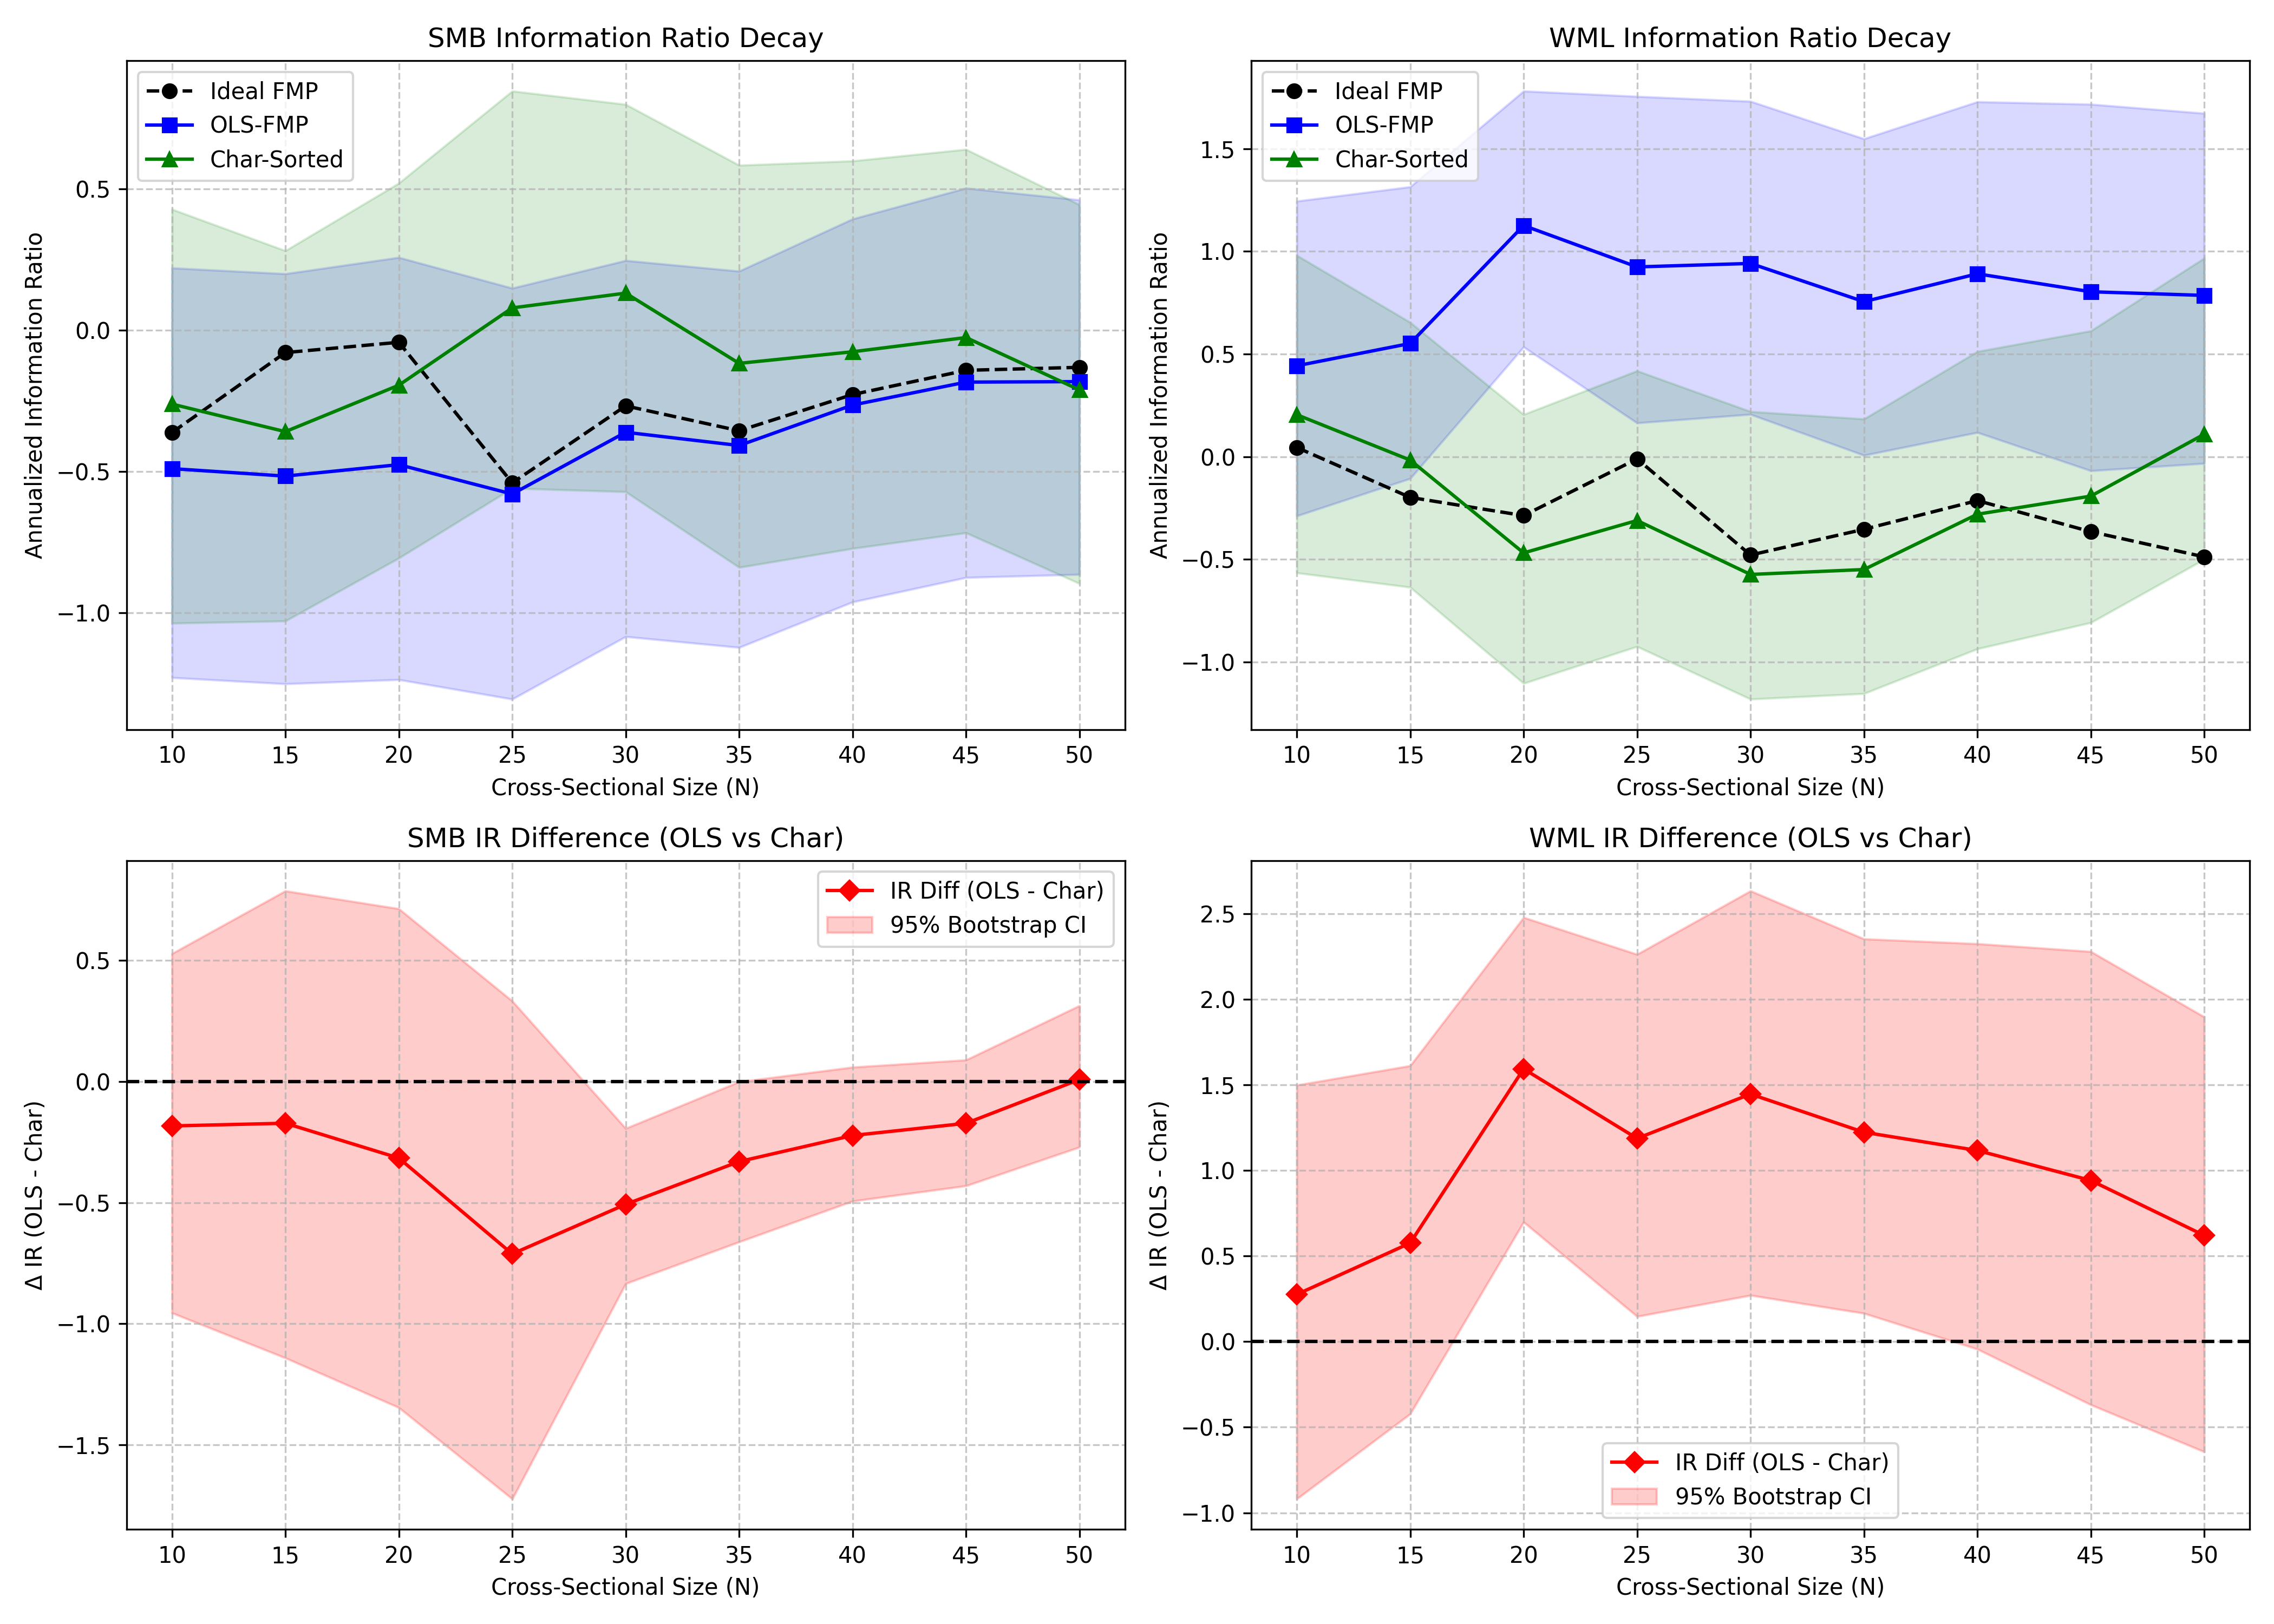
\includegraphics[width=\textwidth]{../input_files/plots/step_5_IR_Decay_Combined_1_20260406_002623.png}
    \caption{Performance comparison of portfolio construction methodologies for the low-Sharpe SMB (left panels) and high-Sharpe WML (right panels) factors as a function of cross-sectional size (N). The top panels plot the Annualized Information Ratio (IR) for Ideal Factor Mimicking Portfolios (Ideal FMP), OLS-estimated FMPs (OLS-FMP), and Characteristic-Sorted portfolios. For the low-Sharpe SMB factor, the OLS-FMP performance attenuates with increasing N due to idiosyncratic noise leakage, whereas the Characteristic-Sorted portfolio remains more stable. Conversely, for the high-Sharpe WML factor, the OLS-FMP successfully captures the premium for N $\ge$ 20, while the Characteristic-Sorted approach fails. The bottom panels display the IR difference between the OLS-FMP and Characteristic-Sorted portfolios ($\Delta$IR = IR\_{OLS} - IR\_{Char}) with 95\% bootstrap confidence intervals, showing that OLS-FMP is statistically superior for WML, while the two methods become statistically indistinguishable for SMB at N $\ge$ 40.}
    \label{fig:image0}
\end{figure*}

\subsection{Idiosyncratic noise leakage as the driver of performance decay}

To understand the mechanism behind the performance decay observed in the SMB OLS-FMP, we decompose the realized portfolio returns into their intended factor component and an unintended idiosyncratic noise component. We quantify the degree of noise contamination using the Noise-to-Signal Ratio (NSR), defined as the variance of the noise component divided by the variance of the factor component.

Figure \ref{fig:image1} shows the evolution of the NSR for the OLS-FMPs. For the low-Sharpe SMB factor, the NSR undergoes a catastrophic explosion as $N$ increases. It begins at 263.8 for $N=10$ and skyrockets to 6572.7 at $N=50$. This demonstrates that for a weak factor signal, the errors in the estimated betas are substantial relative to the true betas. As more assets with poorly estimated loadings are included in the cross-sectional regression, the resulting portfolio weights increasingly amplify idiosyncratic noise, causing the factor signal to be completely overwhelmed.

In stark contrast, the high-Sharpe WML factor exhibits robustness against this degradation. Its NSR remains relatively contained, improving from 511.7 at $N=10$ to 301.9 at $N=50$. The strong true premium of the WML factor provides a sufficient "signal buffer," ensuring that even with estimation errors, the factor component of the portfolio's return remains potent relative to the noise component. This finding confirms that the factor's intrinsic Sharpe ratio is a key determinant of an FMP's vulnerability to idiosyncratic volatility leakage in small-$N$ settings.

\begin{figure}[h!]
    \centering
    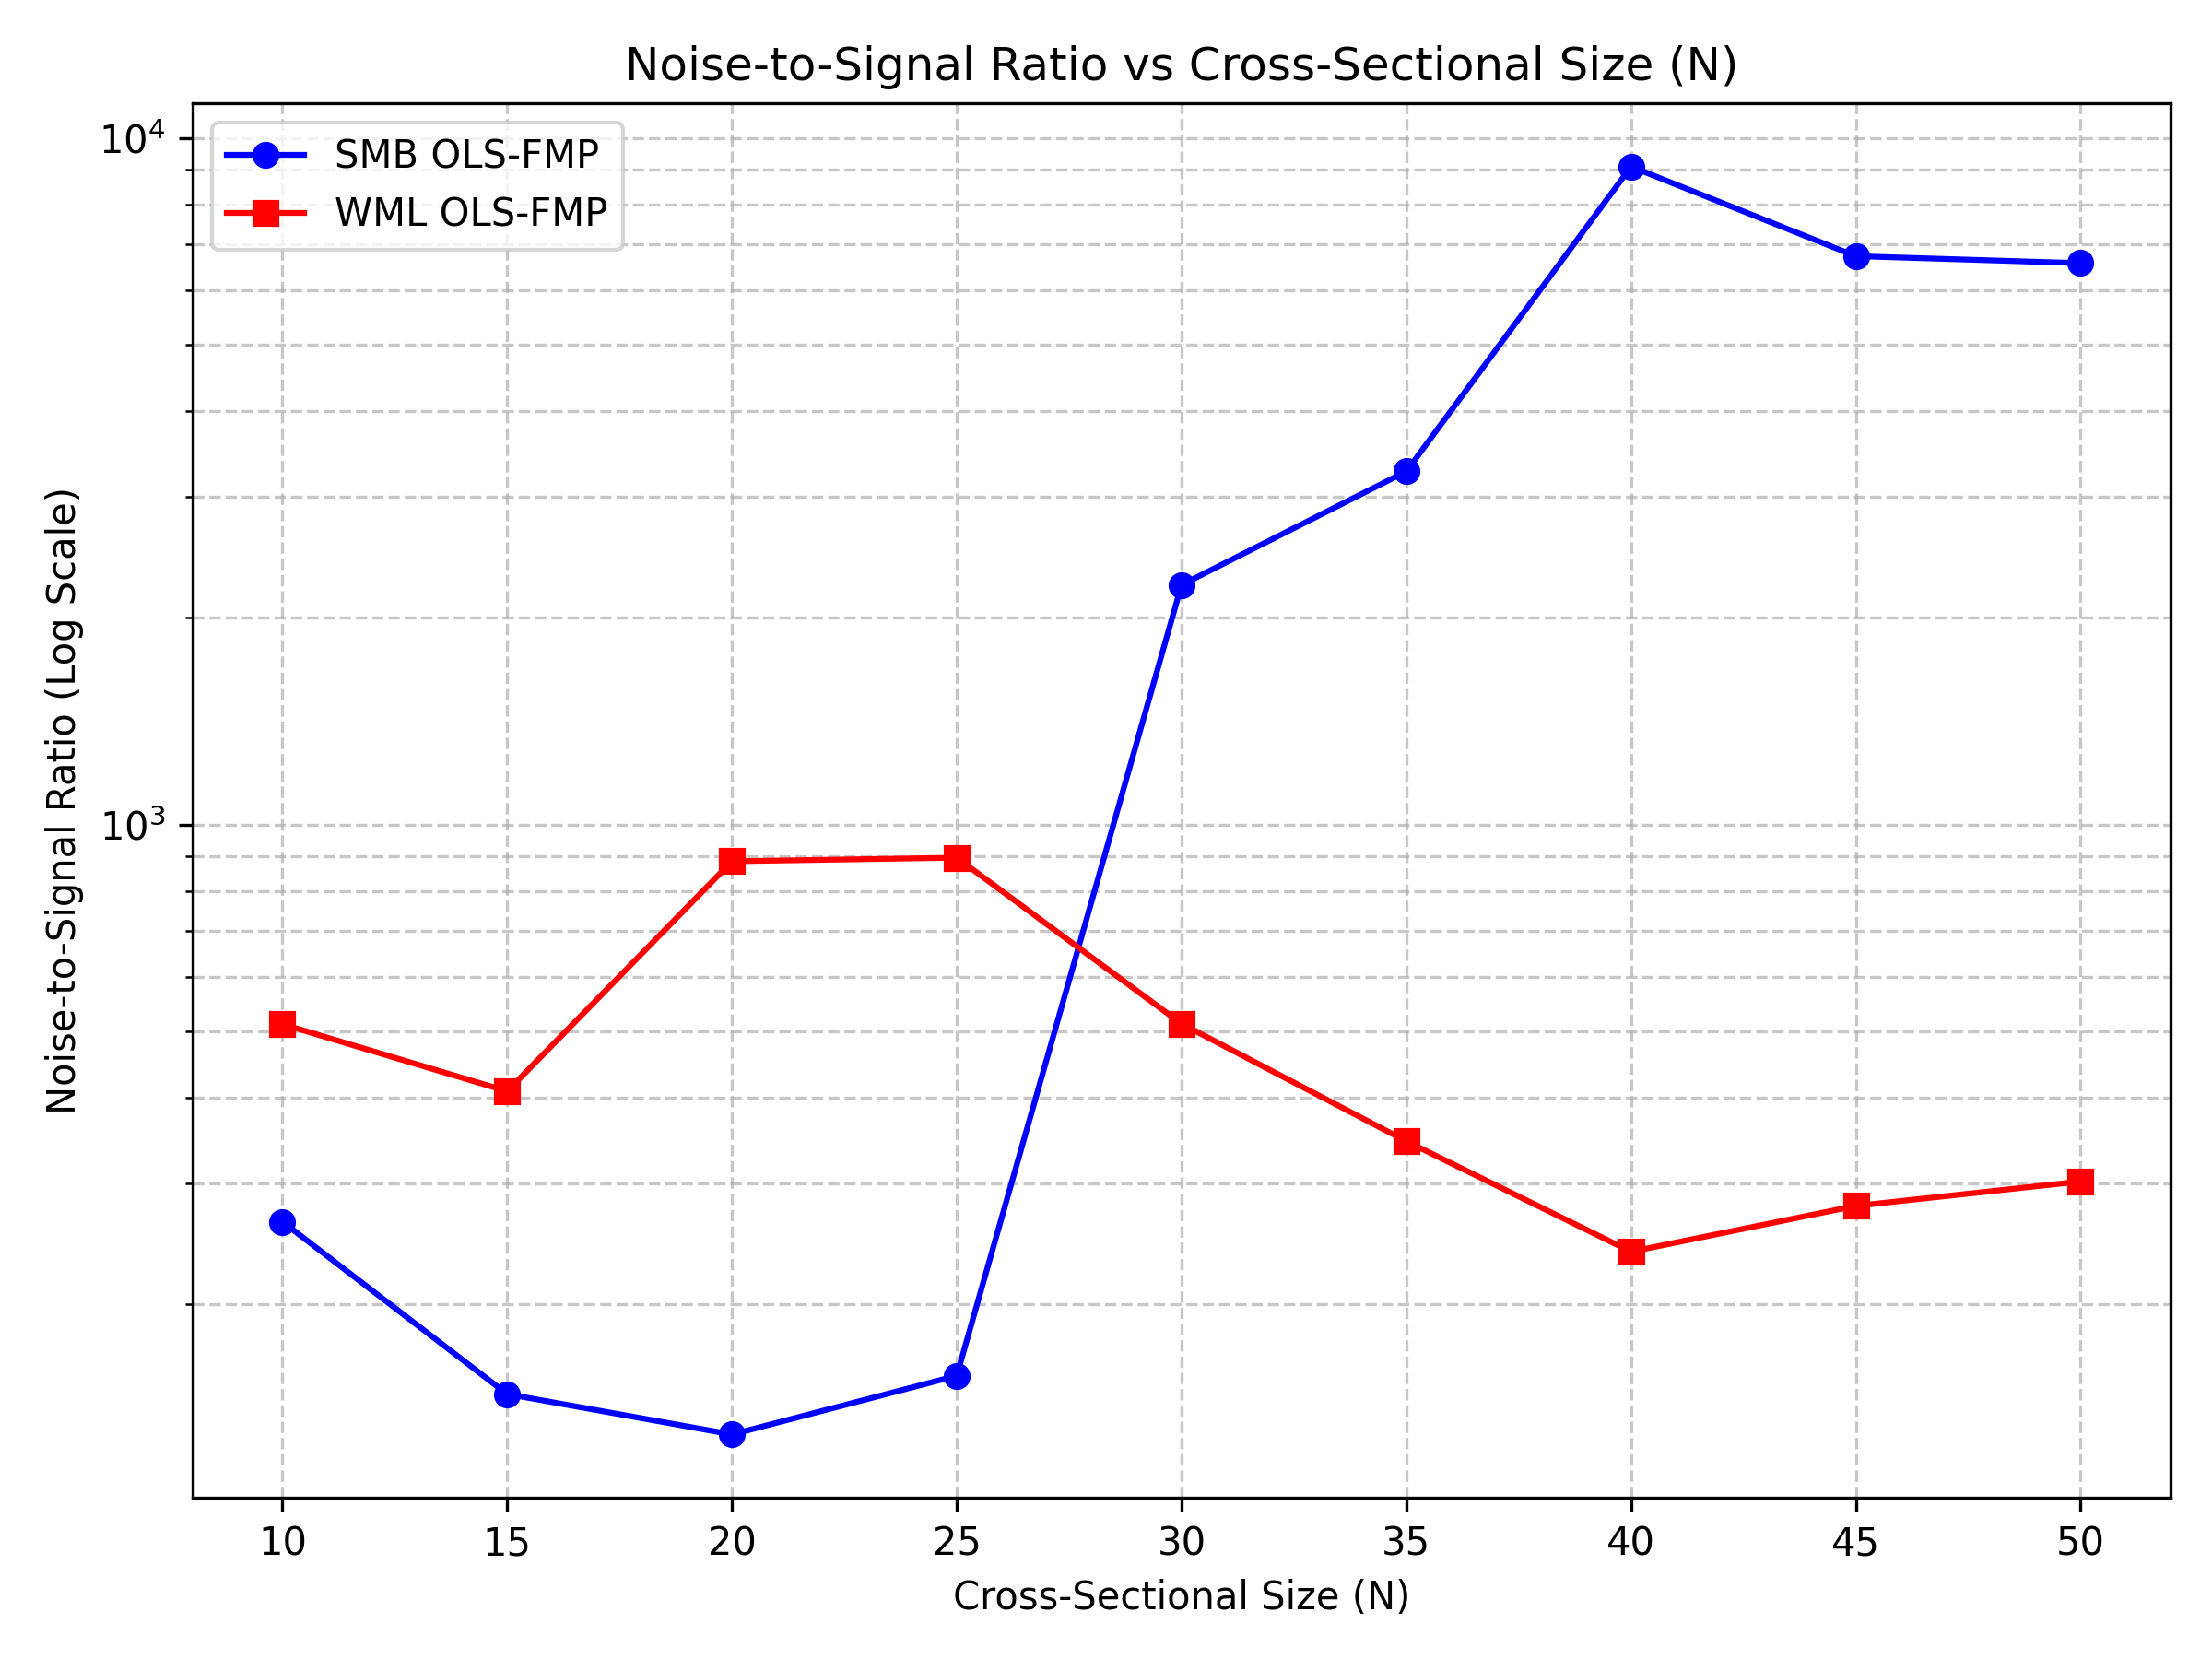
\includegraphics[width=0.5\textwidth]{../input_files/plots/step_5_Noise_to_Signal_Ratio_2_20260406_002623.png}
    \caption{Evolution of the Noise-to-Signal Ratio (NSR) on a logarithmic scale for OLS-estimated Factor Mimicking Portfolios (OLS-FMP) as a function of cross-sectional size (N). For the low-Sharpe SMB factor, the NSR demonstrates a catastrophic increase from 263.8 at N=10 to 6572.7 at N=50, indicating that idiosyncratic volatility leakage from noisy beta estimates overwhelms the factor signal as the cross-section expands. In contrast, the high-Sharpe WML factor shows signal robustness, with its NSR improving from 511.7 to 301.9, highlighting that a strong true premium provides a buffer against estimation error degradation.}
    \label{fig:image1}
\end{figure}

\subsection{Statistical thresholds for factor recovery}

Finally, we establish the statistical significance of our findings by computing Newey-West t-statistics for the IRs and using a block bootstrap to generate 95\% confidence intervals for the performance difference between the OLS-FMP and Characteristic-Sorted portfolios ($\Delta \text{IR} = \text{IR}_{\text{OLS}} - \text{IR}_{\text{Char}}$). Given our 84-month out-of-sample period, an absolute IR greater than approximately 0.74 is required to be statistically different from zero at the 95\% confidence level.

For the low-Sharpe SMB factor, the OLS-FMP's IR never reaches this significance threshold for any cross-sectional size $N \in [10, 50]$. The catastrophic noise leakage documented in Figure \ref{fig:image1} ensures that the estimated premium is statistically indistinguishable from zero. This implies that in a high-noise environment, a weak factor signal cannot be reliably recovered using OLS-FMPs constructed from small cross-sections.

For the high-Sharpe WML factor, a clear threshold emerges. The OLS-FMP's IR is not statistically significant for $N=10$ or $N=15$. However, at $N=20$, the IR jumps to 1.126, decisively crossing the significance threshold. The premium remains statistically significant for all $N \ge 20$, establishing a minimum cross-sectional breadth of 20 assets for reliable recovery of this high-Sharpe factor.

The comparison between methodologies, shown in the bottom panels of Figure \ref{fig:image0}, further clarifies the practical implications. For the WML factor, the OLS-FMP is statistically superior to the misspecified Characteristic-Sorted portfolio for nearly all $N \ge 20$. For the SMB factor, the conclusion is more nuanced. While the OLS-FMP is not statistically worse than the Characteristic-Sorted portfolio, the two methods become statistically indistinguishable for $N \ge 40$, as the 95\% confidence interval for their performance difference contains zero. Given that the Characteristic-Sorted portfolio provides a more accurate point estimate of the true factor premium at larger $N$, it represents the more robust and reliable choice for low-Sharpe factors in these data-constrained settings.

\section{Conclusions}
\label{sec:conclusions}
This paper investigated the reliability of factor mimicking portfolios (FMPs) when constructed from small cross-sections of assets, a setting where uncompensated idiosyncratic noise can overwhelm the target factor signal. To quantify this performance degradation, we employed a simulated panel dataset with a known ground-truth data generating process, allowing for a precise decomposition of portfolio returns into their intended factor and unintended noise components. By systematically varying the number of assets ($N$ from 10 to 50), we compared the efficacy of FMPs estimated via Ordinary Least Squares (OLS) against simpler characteristic-sorted portfolios for two distinct factor archetypes: a low-Sharpe factor (SMB) and a high-Sharpe factor (WML).

Our results reveal a critical interaction between a factor's intrinsic signal strength and the optimal portfolio construction methodology. For the low-Sharpe SMB factor, the statistical complexity of the OLS-FMP proved detrimental. We found that increasing the cross-sectional size paradoxically amplified idiosyncratic noise leakage, causing the estimated premium to be statistically indistinguishable from zero across all sample sizes. In this high-noise, low-signal regime, the structurally simpler characteristic-sorted portfolio provided a more stable and robust estimate of the true factor premium.

Conversely, for the high-Sharpe WML factor, the OLS-FMP successfully isolated a statistically significant premium, but only once the asset universe reached a minimum breadth. We identified a clear threshold at a cross-sectional size of $N=20$, below which the factor signal could not be reliably recovered. For $N \ge 20$, the OLS-FMP decisively outperformed the characteristic-sorted portfolio, which was shown to be structurally misspecified for this factor's data generating process.

From these findings, we have learned that the minimum data requirements for reliable factor replication are not absolute but are contingent on the factor's underlying Sharpe ratio. In high-noise, small-N environments, there is a crucial trade-off between statistical estimation and structural portfolio design. For factors with a weak signal, simpler heuristic methods like characteristic sorting can be more robust than statistically sophisticated FMPs that are prone to amplifying estimation error. For factors with a strong signal, OLS-FMPs can be highly effective, but a minimum threshold of cross-sectional diversification is necessary to ensure the factor signal dominates the noise. This study provides a quantitative framework for understanding the practical limits of factor investing in data-constrained settings.


\bibliography{bibliography}{}
\bibliographystyle{unsrt}

\end{document}
